\chapter{Methodology}
The software methodology used to develop this project will be described in this
chapter. Agile methodologies have been used to drive Alcaudon's development.

Agile methodologies help organizing software development life cycle. They are
focused on iterative development and adaptability. The term was coined during
the early 2000s in the \textit{Agile Manifesto}\cite{manifesto}. The manifesto
has this set of principles:

\begin{itemize}
\item Individuals and interactions over processes and tools
\item Working software over comprehensive documentation
\item Customer collaboration over contract negotiation
\item Responding to change over following a plan
\end{itemize}


\begin{figure}
  \centering
  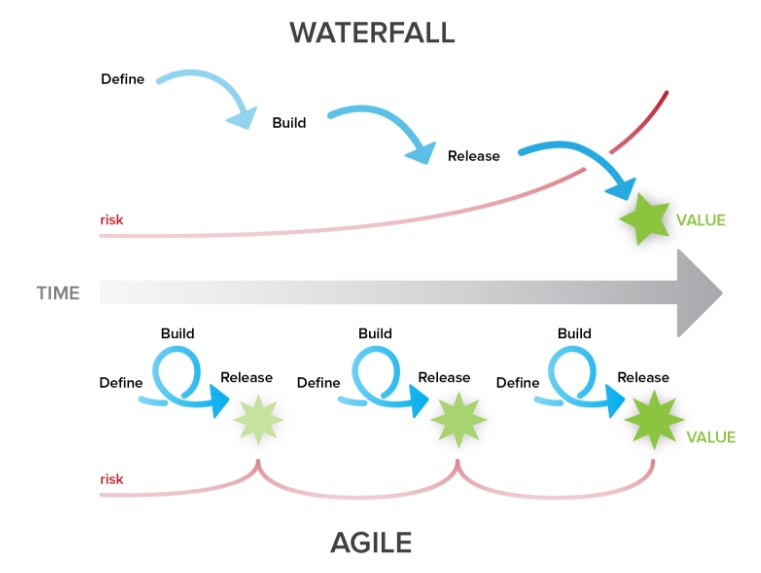
\includegraphics[width=0.8\textwidth]{agile.jpg}
  \caption{Waterfall vs Agile Methodologies\cite{waterfall}}
  \label{fig:waterfall}
\end{figure}

The main goal of these methodologies is to improve communications between all
the stakeholders in a project. This focus on continuous communications reduces
risks and provides value since the very beginning of the project. One of the
outcomes of this iterative open process is a reduction in the costs of the
changes. This differs totally from rigid methodologies such as waterfall where
the customer is taken apart from the project until the very end, skyrocketing
the costs of change as shown in Figure~\ref{fig:waterfall}.

Agile methodologies have become popular during the last 10 years, therefore there
are many agile frameworks that follow the previously enumerated principles. The
most popular ones are:
\begin{itemize}
\item SCRUM\cite{scrum}: Framework that allows teams to develop complex
  adaptive software delivering value as soon as possible.
\item eXtreme Programming\cite{xp}: Lightweight methodology for small-medium
  sized software development teams in scenarios where requirements change often
  or are vague.
\item Kanban\cite{kanban}: Inspired by the work of Toyota during the 1940s to improve
  factory resource utilization, this lightweight methodology also minimizes the processes
  around development. It is focused on having a set of features to be done and delivering
  them as soon as possible. It is a good fit for startup teams.
\end{itemize}

Since Alcaudon's requirements were not clear from the start agile methodologies
provided the optimal framework. In particular, eXtreme Programming was chosen
due to the team's small size and the expected requirement changes.

\section{eXtreme Programming}

\begin{figure}
  \centering
  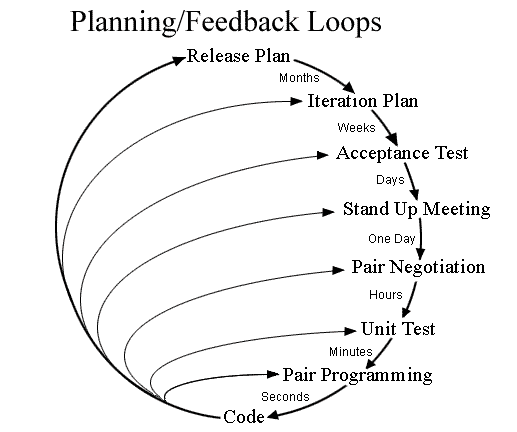
\includegraphics[width=0.6\textwidth]{xp.png}
  \caption{Extreme Programming feedback diagram\cite{xp}}
  \label{fig:xp}
\end{figure}

This methodology proposes a feedback/release cycle as shown in Figure~\ref{fig:xp} and a set of
practices\cite{xp}:

\begin{enumerate}
\item \textit{The planning game}: The scope, priority and date of releases
  should be agreed between business and technical team, adapting them in the
  face of unplanned events. Neither business nor technical parties involved have
  more weight than the other when planning next releases. This is why
  communication is one of the key principles in this methodology. In Alcaudon
  the business team was represented by the advisor, \textit{David Villa Alises},
  and the technical team by the author.
\item Small releases: Every release should be as small as possible providing the
  maximum business value. Alcaudon is released continuously, meaning that it has
  adopted Continuous Deployment\cite{cd} techniques. Every commit pushed to the
  master branch, Travis CI (footnote) launches a continuous delivery pipeline
  that runs tests, builds and publishes an usable version of Alcaudon as docker
  containers and a snapshot version of the libraries to Maven central. This
  practice allows Alcaudon's process to bring value as soon as possible.
  Moreover, it reduces risks, thus contributing to build a more efficient and
  robust system.
\item \textit{Metaphor}: A common language between different participants in the
  project should be use. This makes communication easier and therefore
  misunderstandings are reduced.
\item Simple design: As defined by\cite{xp}, a simple design follows these rules:
  \begin{enumerate}
  \item All tests pass.
  \item There is no duplicated logic.
  \item States every intention important to the programmers.
  \item Has the fewest possible classes, methods and functions.
  \end{enumerate}
  Alcaudon follows these principles. Consequently, the risks associated to
  changes are minimized.
\item Testing: In XP there is a strong bias towards writing tests for all the
  created functionalities, both unit and functional tests. This practice creates
  a stronger confidence in programmers when they need to change their code.
  Alcaudon has been tested broadly, using unit, integration and property based
  testing. Having a good testing coverage has helped to keep developing the
  system with confidence in its correctness, since this project can not be
  easily tested manually.
\item Refactoring: Given the previous principle of \textit{simple design},
  continuous design refinement via refactoring is a key concept in XP.
  Refactoring helps to keep control of complexity iterating over software
  design, reducing risks in future changes. During the development of this
  project, there have been some refactors that improved the design of certain
  modules. Following this principle has been crucial to improve the system's
  architecture.
\item Pair programming: In this methodology there is a preference towards programming
  in pairs. Different points of view can improve the final design and spot
  possible failures that otherwise would have taken longer to detect. This
  principle does not apply to Alcaudon since it is an individual project.
\item Continuous Integration: Code should be integrated and tested every few
  hours. This practice helps to avoid working too long in a big feature, making
  it harder to integrate later. Again, XP is favoring risk reduction with this
  set of practices. As described before, Alcaudon uses Travis CI as continuous
  integration server, for every commit to master the project is built and
  tested.
\item On-site customer: XP accentuates the importance of communications. A
  domain expert, i.e. an user, should be available to answer questions about the
  business and set small scale priorities. Having this person accessible, saves
  time when developers are not familiar with some details about the domain, therefore
  reducing risks.
\item Coding standards: Every project should have coding standards so the
  differences in style among the code written by the team are minimized. An
  example could be a code linter, so if there is a deviation in the defined
  style the programmer will be warned. There are more sophisticated tools to
  define standards, such as code quality measurements tools. These metrics can
  be added in the continuous integration pipeline. if the added code does not
  comply with them, the build is marked as failed. This project uses a code
  linter and advanced compiler warnings (such as unused code, deprecated APIs,
  etc), therefore the coding style is uniform.
\end{enumerate}

\subsection{eXtreme Programming applied to this project}

This section describes the different releases done during the development of
Alcaudon. As it has been stated before, Continuous Deployment has been
implemented, so there has been a production ready release after every code
change. For simplicity this section will describe release cycles with blocks of
features.

\subsubsection{Release 1: State of the art analysis}
\begin{itemize}
\item \textit{Agreed goal}: Distributed data processing systems State of the art analysis.
  \item \textit{Deliverable}: Document describing existing solutions in the
    distributed data processing space as well as recent developments from
    different related conferences such as, VLDB, SIGMOD and OSDI.
\end{itemize}

\subsubsection{Release 2: Technology selection}
\begin{itemize}
\item \textit{Agreed goal}: Given the findings from the previous release,
  investigate suitable technologies to implement a distributed data processing
  system.
\item \textit{Deliverable}: After some investigation and tests two languages
  were chosen, Erlang and Scala. Both implement the actor model. Erlang has been
  proven to be production ready, but according to TIOBE\cite{tiobe} its usage is
  not ample. On the other hand, Scala seems to be quite popular among the data
  processing community. After some discussion with business stakeholders, Scala
  was chosen due to its inter-operability with Java and notoriety among
  developers.
\end{itemize}

\subsubsection{Release 3: Computation, timer, source and sink API definitions}
\begin{itemize}
\item \textit{Agreed goal}: Define the public interface that customers will use
  to implement their computations and timers as well as sources and sinks.
\item \textit{Deliverable}: During this release cycle, communication between the
  different participants in the project was quite productive. A first proposal
  was sent to the domain expert, the advisor in this project. This first version
  did not take into account certain details that were key to the project. Given
  the early feedback, it was possible to react quickly and present a new
  computation API that contained less details about the implementation,
  providing a better abstraction.
\end{itemize}

\subsubsection{Release 4: Dataflow builder development}
\begin{itemize}
\item \textit{Agreed goal}: Develop a first dataflow builder version where the
  user can define a dataflow topology.
\item \textit{Deliverable}: During this release an usable dataflow builder was
  delivered. Alcaudon users were able to build their own computation topologies.
  This allowed to start testing how usable the interface was and with the given
  feedback improve the initial designs.
\end{itemize}

\subsubsection{Release 5: First computation execution engine version development}
\begin{itemize}
\item \textit{Agreed goal}: Implement the first version for the computation
  execution engine.
\item \textit{Deliverable}: Since Dataflow builder was developed during the previous
  release, the next natural step was to implement the computation executor.
  During this release a simplified engine version was released, making possible
  to test simple computations.
\end{itemize}

\subsubsection{Release 6: Computation execution guarantees development}
\begin{itemize}
\item \textit{Agreed goal}: Implement means to provide fault-tolerant computation executions.
\item \textit{Deliverable}: One of the Alcaudon goals is to be fault-tolerant.
  The outcome of this release cycle was fully tested computation engine that
  complies with the fault-tolerant agreed requirements.
\end{itemize}

\subsubsection{Release 7: Timer execution engine development}
\begin{itemize}
\item \textit{Agreed goal}: Implement fixed and watermark based timers.
\item \textit{Deliverable}: Alcaudon works with unbounded data-sets, hence a way
  to emit partial results should be provided. In this release, fixed timers and watermark
  timers were released. Watermarks were developed using CRDT's.
\end{itemize}

\subsubsection{Release 8: Generic serialization library development}
\begin{itemize}
\item \textit{Agreed goal}: Develop generic serialization library for Algebraic
  Data Types.
\item \textit{Deliverable}: Data travels around Alcaudon as an array of bytes.
  There are many serialization formats to transform high level entities to
  binary data. However, for simplicity, a generic serialization library has been
  developed. This library is able to, given an Algebraic Data Type, create a
  serializer/de-serializer using scala implicit induction during compile time.
\end{itemize}

\subsubsection{Release 9: Stream entity implementation}
\begin{itemize}
\item \textit{Agreed goal}: Implement an Stream representation so data can be
  published and consumed from it. Published data should be durable.
\item \textit{Deliverable}: Computations subscribe to streams, in this release a
  durable stream representation was implemented so consumers and publishers can
  consume and publish stream records. During this release given the changes
  appeared during the design of the stream entity, some refactors in the
  computation execution engine were done.
\end{itemize}

\subsubsection{Release 9: Library manager implementation}
\begin{itemize}
\item \textit{Agreed goal}: Implement a subsystem that enables dynamic load of
  arbitrary user code into remote Alcaudon workers.
\item \textit{Deliverable}: A module to load arbitrary user code was developed.
  It is backed by a cloud object storage\footnote{https://aws.amazon.com/s3/},
  and allows dynamic load of user code.
\end{itemize}

\subsubsection{Release 10: Distributed architecture design}
\begin{itemize}
\item \textit{Agreed goal}: Design a resilient distributed architecture that
  allows remote work distribution for the system.
\item \textit{Deliverable}: During this release some requirement changes were brought
  by the business side due to a bug in the stream implementation. Given the urgency
  of those changes, just a partial design was done.
\end{itemize}

\subsubsection{Release 11: Distributed architecture implementation}
\begin{itemize}
\item \textit{Agreed goal}: Finish the first design for the distributed
  architecture and implement a prototype.
\item \textit{Deliverable}: In this release, a first version for the distributed
  architecture was developed. The idea was to keep developing during the next
  release cycles.
\end{itemize}

\subsubsection{Release 12: Implement job scheduling policy}
\begin{itemize}
\item \textit{Agreed goal}: Implement computation scheduling to distribute the
  dataflow topology in the most optimal possible configuration.
\item \textit{Deliverable}: Due to the time constraints, during this release it
  was decided to use available tools to solve the flexible job-shop scheduling
  problem. In this case, a set of optimization tools provided by Google were
  used.
\end{itemize}

\subsubsection{Release 13: Implement tools that allows monitoring the system}
\begin{itemize}
\item \textit{Agreed goal}: Implement tools or adopt external tools that allow
  observe the behavior of the system.
\item \textit{Deliverable}: After some investigation it was agreed to used both
  an external system to facilitate observability, Prometheus and implement some
  tools to track how the system is performing.
\end{itemize}

\subsubsection{Release 14: implement some sources and sinks}
\begin{itemize}
\item \textit{Agreed goal}: Provide some default implementations of sources and
  sinks, such as TCP sockets or Twitter streaming api.
\item \textit{Deliverable}: During this release the agreed goals were implemented. Given
  that the system needed some improvements this latest release was used also to refactor
  some modules of the system to give them more reliability.
\end{itemize}

\section{Development technologies}

There are many technologies available to develop information systems. Different
paradigms, different environments, etc. For Alcaudon, working with the JVM
seemed to be a good choice. It is one of the most advanced language virtual
machines in the market, with outstanding implementations such as
OpenJDK\footnote{http://openjdk.java.net/} or
Zing\footnote{https://www.azul.com/products/zing/virtual-machine/}. The
available ecosystem of tools and libraries covers many domains. There are
multiple implementations for state of the art data structures used in this
project such as cuckoo filters\cite{cuckoo}. Another reason to choose the JVM
was the inter-operability between different languages such as Scala and Java.
Scala has been chosen as the principal programming language. It is an hybrid
language that allows programmer to use functional and object oriented
programming paradigms. This design is interesting, it allows to combine the best
of both worlds, providing tools to work with functional constructs such as
monadic composition or use more object oriented tools such as traits.

In the database space, Cassandra has been chosen as the principal data store due
to it is designed with high availability and scalability in mind. This choice
provide good grounds to guarantee data durability within the system. For storing
time series data, Prometheus has been chosen due to its high scalability and
performance querying historic data.

Other tool used to develop Alcaudon has been TravisCI, a cloud continuous
integration service. Using a service that is fully integrated with git made the
set-up of the CD pipeline easier.

\section{Tools}

In this section tools used to develop Alcuadon will be presented. 

\subsection{Hardware}

The only physical hardware used to develop this project have been a laptop. For
deploying the system, Amazon Web Services has been used. All the incurring costs
for testing have been assumed by the author of this project.

\begin{itemize}
  \item Dell XPS 13 with Intel\textregistered Core\texttrademark i5 2.5GHz
    processor 8GB RAM DDR3 and 128GB SSD hard drive.
  \item Amazon Web Services provided servers with different specifications.
\end{itemize}

\subsection{Software}

\begin{itemize}
  \item Operating Systems
    \begin{itemize}
        \item Debian 8 Jessie\footnote{https://www.debian.org/index.es.html}.
          Operating system used to develop the system and the documentation.
        \item CoreOS\footnote{https://www.coreos.com/}. Minimal linux operating
          system that supports container systems out of the box. Used to deploy
          Alcaudon.
    \end{itemize}

  \item Languages
    \begin{itemize}
      \item Scala\footnote{https://www.scala-lang.org/}. Hybrid Functional and
        Object Oriented programming language used to develop the system.
      \item \LaTeX{}\footnote{https://www.latex-project.org/}. Used language to
        write the documentation.
    \end{itemize}

  \item Frameworks, libraries and databases
    \begin{itemize}
      \item Akka\footnote{https://akka.io}. Toolkit to develop actor based
        systems. Most of the system relies on the actor model. The following
        extensions have been used:
        \begin{itemize}
        \item akka-cluster
        \item akka-persistence
        \item akka-distributed-data
        \end{itemize}
      \item Shapeless\footnote{https://github.com/milessabin/shapeless}. Generic
        programming for Scala used to develop generic serializers.
      \item Apache Cassandra\footnote{http://cassandra.apache.org/}. Open source
        database aimed for scalability.
      \item Scala Graph\footnote{http://www.scala-graph.org/}. Graph data
        structure implementation for Scala.
      \item
        CuckooFilter4j\footnote{https://github.com/MGunlogson/CuckooFilter4J}.
        High performance Java implementation of a Cuckoo filter.
      \item ScalaCheck\footnote{https://www.scalacheck.org/}. Property based
        testing library for Scala.
      \item ScalaTest\footnote{http://www.scalatest.org/}. Testing framework for
        Scala.
      \item Kryo\footnote{https://github.com/EsotericSoftware/kryo}. Fast efficient serialization
        framework for the JVM.
      \item Prometheus\footnote{https://github.com/EsotericSoftware/kryo}. Open
        source time series database used for monitoring.
      \item Google Optimization
        Tools\footnote{https://github.com/google/or-tools}. Google Optimization
        Tools (OR-Tools) is a fast and portable software suite for solving
        combinatorial optimization problems. Used for job scheduling.
    \end{itemize}

  \item Tools
    \begin{itemize}
      \item sbt\footnote{http://www.scala-sbt.org/}. Build tool for Scala.
      \item Emacs \footnote{https://atom.io/}. Text editor used to program the system.
      \item Git\footnote{https://git-scm.com/}. Distributed version control system.
      \item TravisCI\footnote{https://www.travis-ci.org/}. Cloud continuous integration service.
      \item Docker\footnote{https://www.docker.com/}. Linux container runtime.
      \item Grafana\footnote{https://grafana.com/}. Open platform for analytics and monitoring.
    \end{itemize}

\end{itemize}
